%% LyX 2.2.2 created this file.  For more info, see http://www.lyx.org/.
%% Do not edit unless you really know what you are doing.
\documentclass[english,handout]{beamer}
\usepackage{mathptmx}
\usepackage{eulervm}
\usepackage[T1]{fontenc}
\usepackage[latin9]{inputenc}
\usepackage{amsmath}
\usepackage{amssymb}
\usepackage{graphicx}

\makeatletter

%%%%%%%%%%%%%%%%%%%%%%%%%%%%%% LyX specific LaTeX commands.
%% A simple dot to overcome graphicx limitations
\newcommand{\lyxdot}{.}


%%%%%%%%%%%%%%%%%%%%%%%%%%%%%% Textclass specific LaTeX commands.
 % this default might be overridden by plain title style
 \newcommand\makebeamertitle{\frame{\maketitle}}%
 % (ERT) argument for the TOC
 \AtBeginDocument{%
   \let\origtableofcontents=\tableofcontents
   \def\tableofcontents{\@ifnextchar[{\origtableofcontents}{\gobbletableofcontents}}
   \def\gobbletableofcontents#1{\origtableofcontents}
 }

%%%%%%%%%%%%%%%%%%%%%%%%%%%%%% User specified LaTeX commands.
\usetheme{CambridgeUS} 
\beamertemplatenavigationsymbolsempty

\AtBeginSection[]{
  \begin{frame}
  \vfill
  \centering
  \begin{beamercolorbox}[sep=8pt,center,shadow=true,rounded=true]{title}
    \usebeamerfont{title}\insertsectionhead\par%
  \end{beamercolorbox}
  \vfill
  \end{frame}
}

\makeatother

\usepackage{babel}
\begin{document}
\global\long\def\reals{\mathbf{R}}
 \global\long\def\integers{\mathbf{Z}}
 \global\long\def\naturals{\mathbf{N}}
 \global\long\def\rationals{\mathbf{Q}}
 \global\long\def\ca{\mathcal{A}}
 \global\long\def\cb{\mathcal{B}}
 \global\long\def\cc{\mathcal{C}}
 \global\long\def\cd{\mathcal{D}}
 \global\long\def\ce{\mathcal{E}}
 \global\long\def\cf{\mathcal{F}}
 \global\long\def\cg{\mathcal{G}}
 \global\long\def\ch{\mathcal{H}}
 \global\long\def\ci{\mathcal{I}}
 \global\long\def\cj{\mathcal{J}}
 \global\long\def\ck{\mathcal{K}}
 \global\long\def\cl{\mathcal{L}}
 \global\long\def\cm{\mathcal{M}}
 \global\long\def\cn{\mathcal{N}}
 \global\long\def\co{\mathcal{O}}
 \global\long\def\cp{\mathcal{P}}
 \global\long\def\cq{\mathcal{Q}}
 \global\long\def\calr{\mathcal{R}}
 \global\long\def\cs{\mathcal{S}}
 \global\long\def\ct{\mathcal{T}}
 \global\long\def\cu{\mathcal{U}}
 \global\long\def\cv{\mathcal{V}}
 \global\long\def\cw{\mathcal{W}}
 \global\long\def\cx{\mathcal{X}}
 \global\long\def\cy{\mathcal{Y}}
 \global\long\def\cz{\mathcal{Z}}
 \global\long\def\ind#1{1(#1)}
 %\newcommand{\pr}{P}
\global\long\def\pr{\mathbb{P}}
 \global\long\def\predsp{\cy}
 %{\hat{\cy}}
\global\long\def\outsp{\cy}

\global\long\def\prxy{P_{\cx\times\cy}}
 \global\long\def\prx{P_{\cx}}
 \global\long\def\prygivenx{P_{\cy\mid\cx}}
 %\newcommand{\ex}{E}
\global\long\def\ex{\mathbb{E}}
 \global\long\def\var{\textrm{Var}}
 \global\long\def\Ind{\mathbf{1}}
 \global\long\def\cov{\textrm{Cov}}
 \global\long\def\sgn{\textrm{sgn}}
 \global\long\def\sign{\textrm{sign}}
 \global\long\def\kl{\textrm{KL}}
 \global\long\def\law{\mathcal{L}}
 \global\long\def\eps{\varepsilon}
 \global\long\def\as{\textrm{ a.s.}}
 \global\long\def\io{\textrm{ i.o.}}
 \global\long\def\ev{\textrm{ ev.}}
 \global\long\def\convd{\stackrel{d}{\to}}
 \global\long\def\eqd{\stackrel{d}{=}}
 \global\long\def\del{\nabla}
 \global\long\def\loss{\ell}
 \global\long\def\risk{R}
 \global\long\def\emprisk{\hat{R}}
 \global\long\def\lossfnl{L}
 \global\long\def\emplossfnl{\hat{L}}
 \global\long\def\empminimizer#1{\hat{#1}^{*}}
 \global\long\def\minimizer#1{#1^{*}}
\global\long\def\optimizer#1{#1^{*}}
 \global\long\def\etal{\textrm{et. al.}}
 \global\long\def\tr{\operatorname{tr}}

\global\long\def\trace{\operatorname{trace}}
 \global\long\def\diag{\text{diag}}
 \global\long\def\rank{\text{rank}}
 \global\long\def\linspan{\text{span}}
 \global\long\def\spn{\text{span}}
 \global\long\def\proj{\text{Proj}}
 \global\long\def\argmax{\operatornamewithlimits{arg\, max}}
 \global\long\def\argmin{\operatornamewithlimits{arg\, min}}

\global\long\def\bfx{\mathbf{x}}
 \global\long\def\bfy{\mathbf{y}}
 \global\long\def\bfl{\mathbf{\lambda}}
 \global\long\def\bfm{\mathbf{\mu}}
 \global\long\def\calL{\mathcal{L}}

\global\long\def\vw{\boldsymbol{w}}
 \global\long\def\vx{\boldsymbol{x}}
 \global\long\def\vxi{\boldsymbol{\xi}}
 \global\long\def\valpha{\boldsymbol{\alpha}}
 \global\long\def\vbeta{\boldsymbol{\beta}}
 \global\long\def\vsigma{\boldsymbol{\sigma}}
\global\long\def\vtheta{\boldsymbol{\theta}}
 \global\long\def\vd{\boldsymbol{d}}
 \global\long\def\vs{\boldsymbol{s}}
 \global\long\def\vt{\boldsymbol{t}}
 \global\long\def\vh{\boldsymbol{h}}
 \global\long\def\ve{\boldsymbol{e}}
 \global\long\def\vf{\boldsymbol{f}}
 \global\long\def\vg{\boldsymbol{g}}
 \global\long\def\vz{\boldsymbol{z}}
 \global\long\def\vk{\boldsymbol{k}}
 \global\long\def\va{\boldsymbol{a}}
 \global\long\def\vb{\boldsymbol{b}}
 \global\long\def\vv{\boldsymbol{v}}
 \global\long\def\vy{\boldsymbol{y}}

\global\long\def\hil{\ch}
 \global\long\def\rkhs{\hil}
 \global\long\def\ber{\text{Ber}}


\title[DS-GA 1003 ]{$K$-Means}

\author{David Rosenberg, Brett Bernstein}

\date{\today}

\institute{New York University}

\makebeamertitle

\section{Intro Question}
\begin{frame}{Intro Question}
  Consider the following probability model for generating data.
  \begin{enumerate}
  \item Roll a weighted $k$-sided die to choose a label
    $z\in\{1,\ldots,k\}$.  Let $\pi$ denote the PMF for the die.
  \item Draw $x\in\reals^d$ randomly from the multivariate normal
    distribution $\cn(\mu_z,\Sigma_z)$.
  \end{enumerate}
  Solve the following questions.
  \begin{enumerate}
  \item What is the joint distribution of $x,z$ given $\pi$ and the
    $\mu_z,\Sigma_z$ values?
  \item Suppose you were given the dataset
    $\cd=\{(x_1,z_1),\ldots,(x_n,z_n)\}$.  How would you estimate the
    die weightings, and the $\mu_z,\Sigma_z$ values?
  \item How would you determine the label for a new datapoint $x$?
  \end{enumerate}
\end{frame}
\begin{frame}{Intro Solution}
  \begin{enumerate}
  \item The joint PDF/PMF is given by
    $$p(x,z) = \pi(z)f(x;\mu_z,\Sigma_z)$$
    where
    $$f(x;\mu_z,\Sigma_z) =
    \frac{1}{\sqrt{|2\pi\Sigma_z|}}\exp\left(-\frac{1}{2}(x-\mu)^T\Sigma^{-1}(x-\mu)\right).$$
  \item We could use maximum likelihood estimation.  Our estimates are
    $$\begin{array}{rcl}
    n_z  & = & \sum_{i=1}^n \Ind(z_i=z) \\
    \hat{\pi}(z) & = & \frac{n_z}{n}\\
    \hat{\mu}_z & = & \frac{1}{n_z}\sum_{i:z_i=z} x_i\\
    \hat{\Sigma}_z & = & \frac{1}{n_z}\sum_{i:z_i=z} (x_i-\hat{\mu}_z)(x_i-\hat{\mu}_z)^T.
    \end{array}$$
  \item $\argmax_z p(x,z)$
  \end{enumerate}
\end{frame}

\section{$K$-Means Clustering}
\begin{frame}{Example: Old Faithful Geyser}

\begin{center}
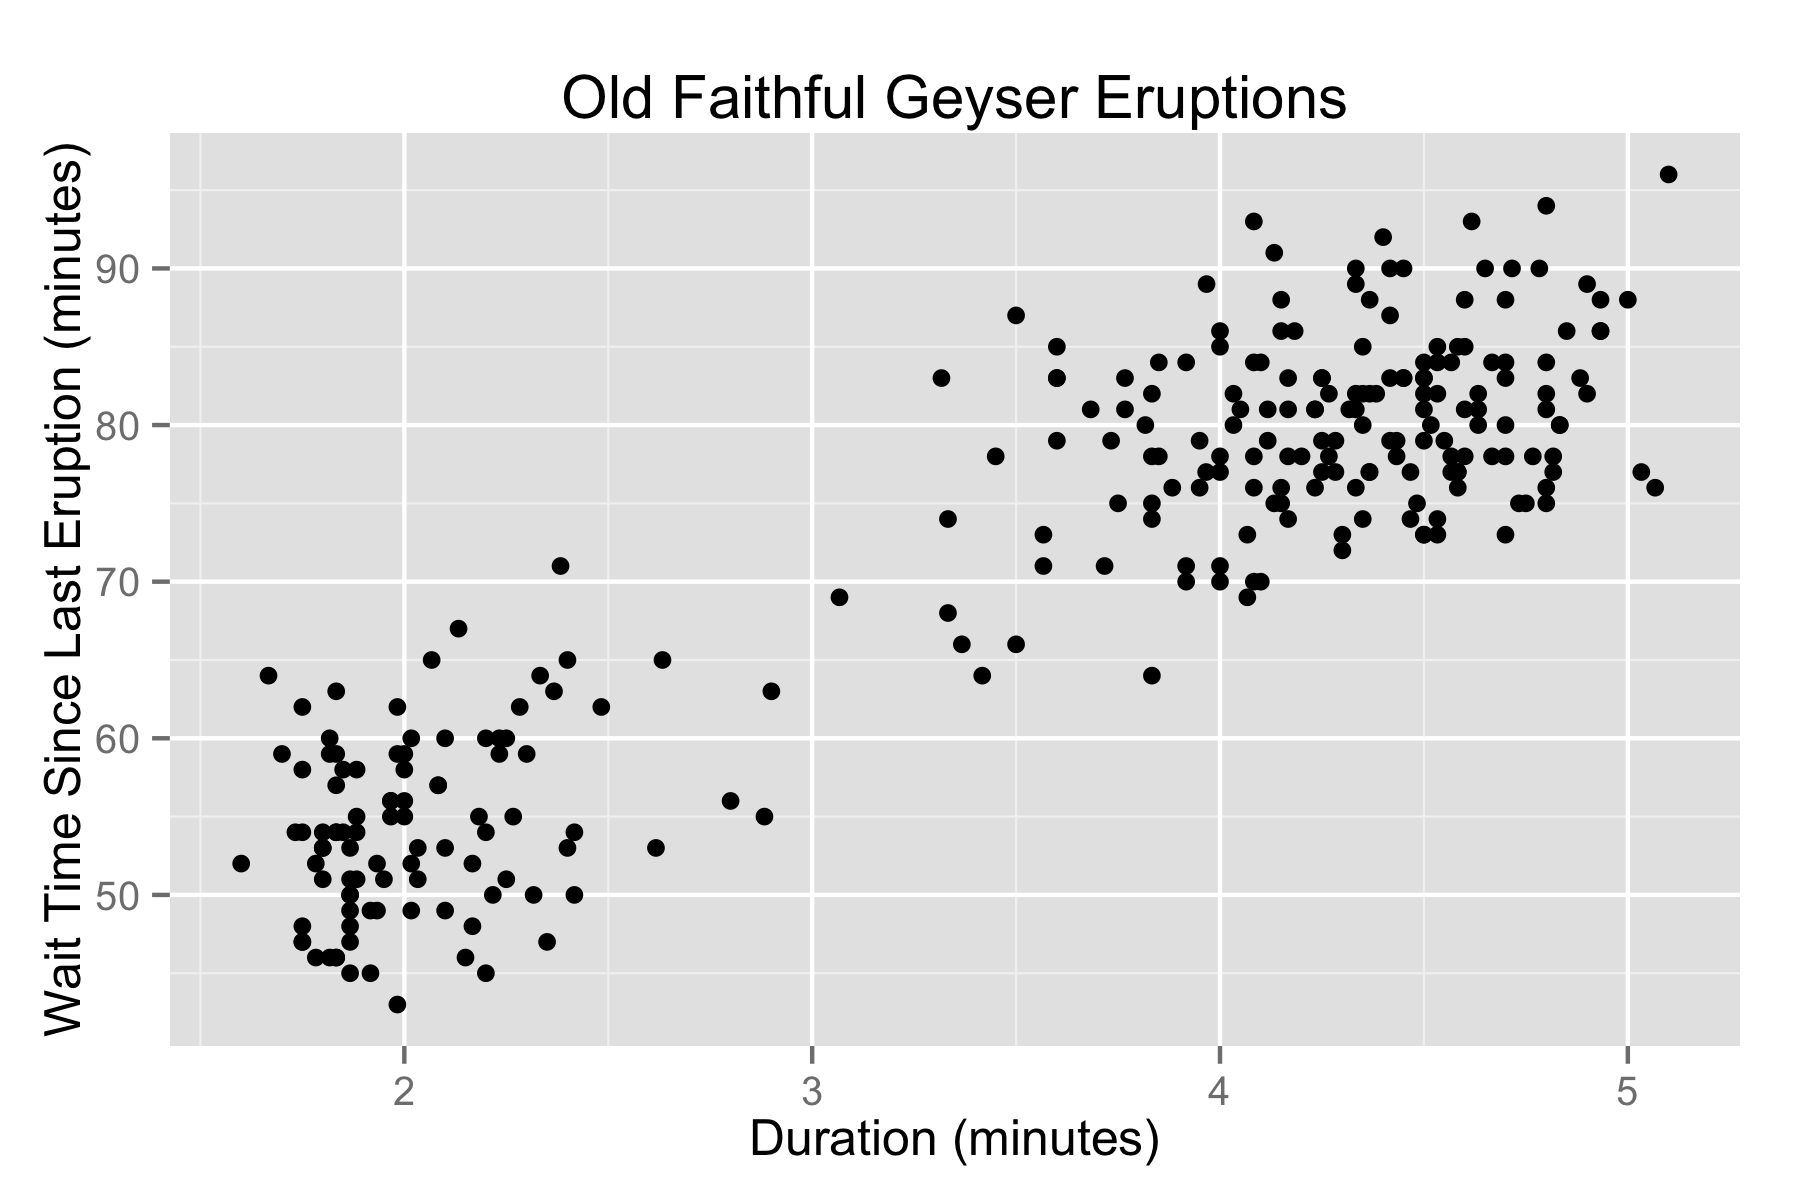
\includegraphics[width=0.65\textwidth]{../Figures/clustering/oldfaithful}
\par\end{center}
\begin{itemize}
\item Looks like two clusters.
\item How to find these clusters algorithmically?
\end{itemize}
\end{frame}

\begin{frame}{$k$-Means: By Example}

\begin{itemize}
\item Standardize the data.
\item Choose two cluster centers.
\end{itemize}
\begin{center}
\includegraphics[height=0.55\textheight]{../Figures/clustering/faithful-9\lyxdot 1a}
\par\end{center}

\let\thefootnote\relax\footnotetext{\tiny{From Bishop's \emph{Pattern recognition and machine learning}, Figure 9.1(a).}}

\end{frame}

\begin{frame}{k-means: by example}

\begin{itemize}
\item Assign each point to closest center.
\end{itemize}
\begin{center}
\includegraphics[height=0.55\textheight]{../Figures/clustering/faithful-9\lyxdot 1b}
\par\end{center}

\let\thefootnote\relax\footnotetext{\tiny{From Bishop's \emph{Pattern recognition and machine learning}, Figure 9.1(b).}}
\end{frame}

\begin{frame}{k-means: by example}

\begin{itemize}
\item Compute new class centers.
\end{itemize}
\begin{center}
\includegraphics[height=0.55\textheight]{../Figures/clustering/faithful-9\lyxdot 1c}
\par\end{center}

\let\thefootnote\relax\footnotetext{\tiny{From Bishop's \emph{Pattern recognition and machine learning}, Figure 9.1(c).}}
\end{frame}

\begin{frame}{k-means: by example}

\begin{itemize}
\item Assign points to closest center.
\end{itemize}
\begin{center}
\includegraphics[height=0.55\textheight]{../Figures/clustering/faithful-9\lyxdot 1d}
\par\end{center}

\let\thefootnote\relax\footnotetext{\tiny{From Bishop's \emph{Pattern recognition and machine learning}, Figure 9.1(d).}}
\end{frame}

\begin{frame}{k-means: by example}

\begin{itemize}
\item Compute cluster centers.
\end{itemize}
\begin{center}
\includegraphics[height=0.55\textheight]{../Figures/clustering/faithful-9\lyxdot 1e}
\par\end{center}

\let\thefootnote\relax\footnotetext{\tiny{From Bishop's \emph{Pattern recognition and machine learning}, Figure 9.1(e).}}
\end{frame}

\begin{frame}{k-means: by example}

\begin{itemize}
\item Iterate until convergence.
\end{itemize}
\begin{center}
\includegraphics[height=0.55\textheight]{../Figures/clustering/faithful-9\lyxdot 1i}
\par\end{center}

\let\thefootnote\relax\footnotetext{\tiny{From Bishop's \emph{Pattern recognition and machine learning}, Figure 9.1(i).}}
\end{frame}

\begin{frame}{$k$-Means Algorithm: Standardizing the data}

\begin{itemize}
\item Without standardizing:
\end{itemize}
\begin{center}
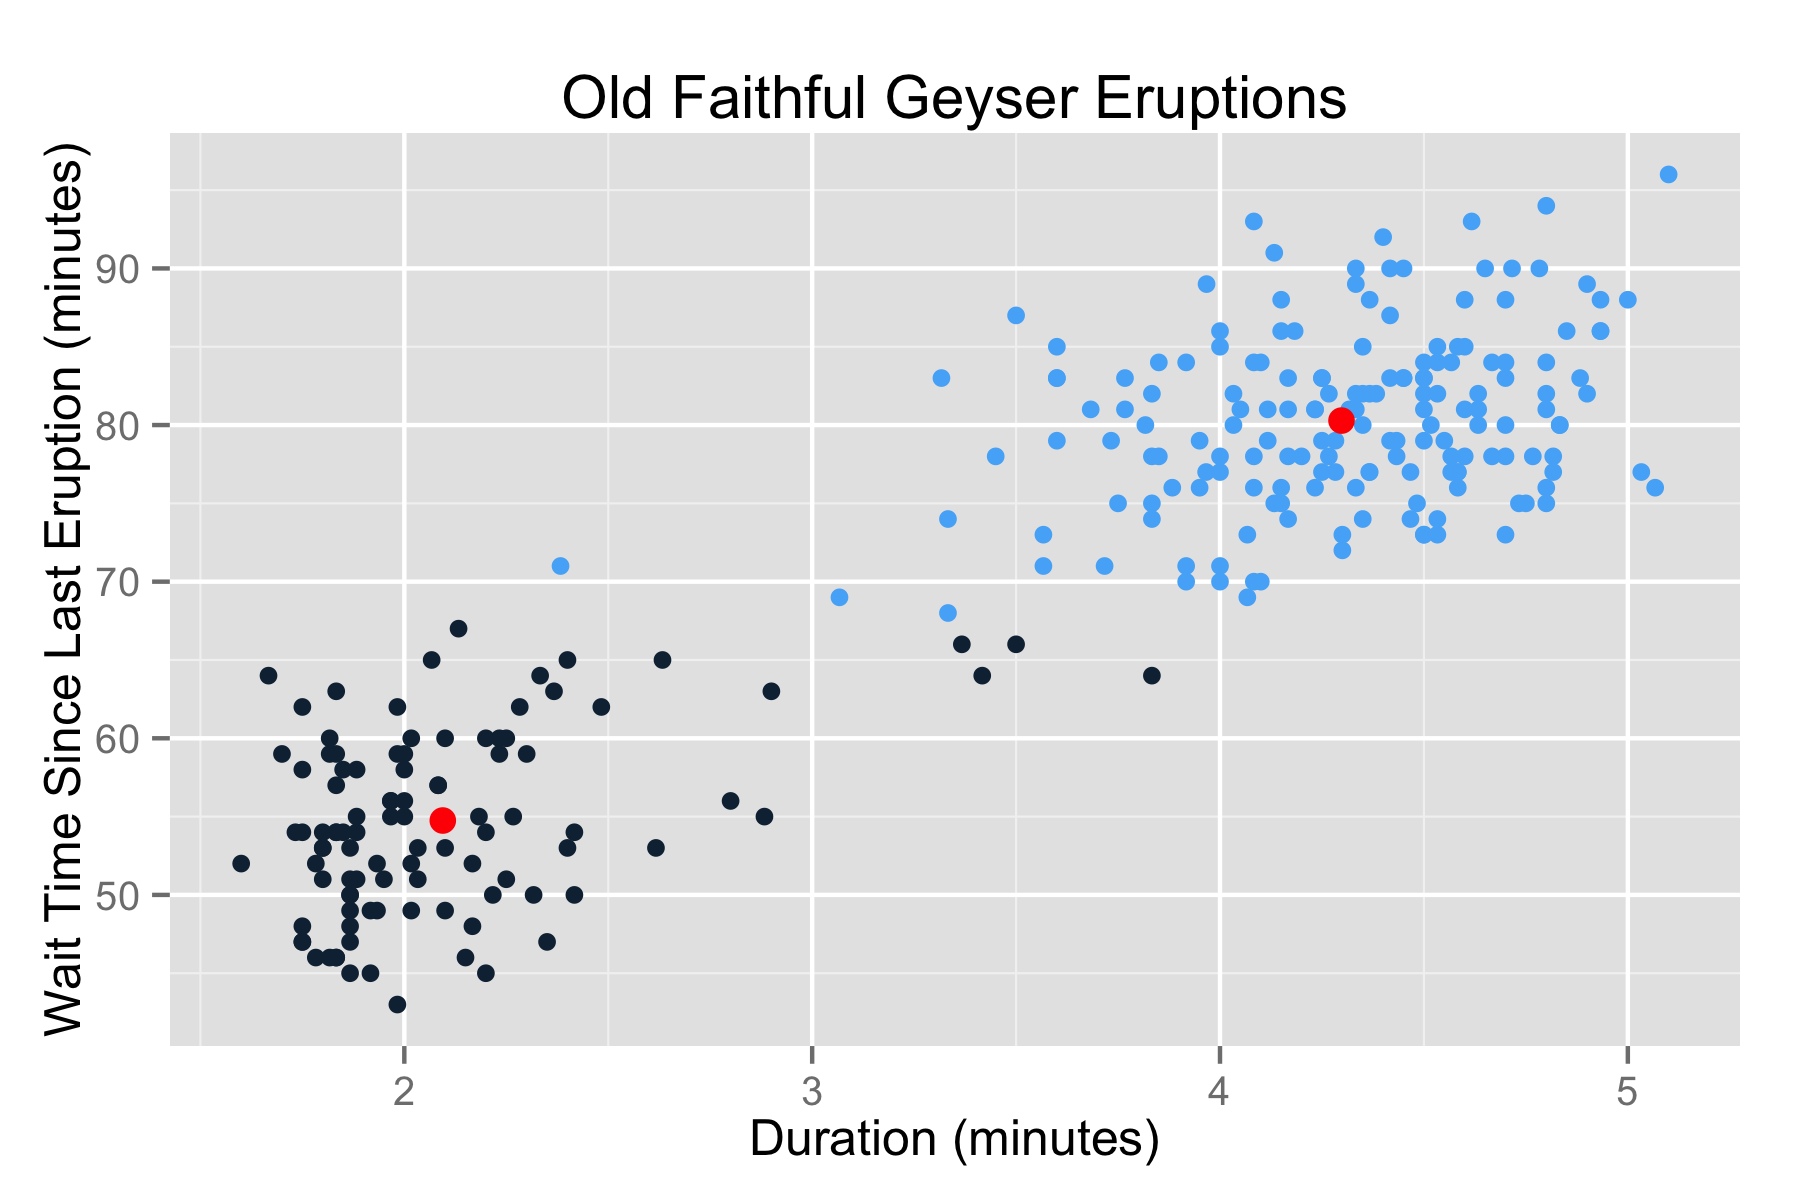
\includegraphics[width=0.65\textwidth]{../Figures/clustering/oldfaithful-clusterNoRescale}
\par\end{center}
\begin{itemize}
\item Blue and black show results of k-means clustering
\item Wait time dominates the distance metric
\end{itemize}
\end{frame}

\begin{frame}{$k$-Means Algorithm: Standardizing the data}

\begin{itemize}
\item With standardizing:
\end{itemize}
\begin{center}
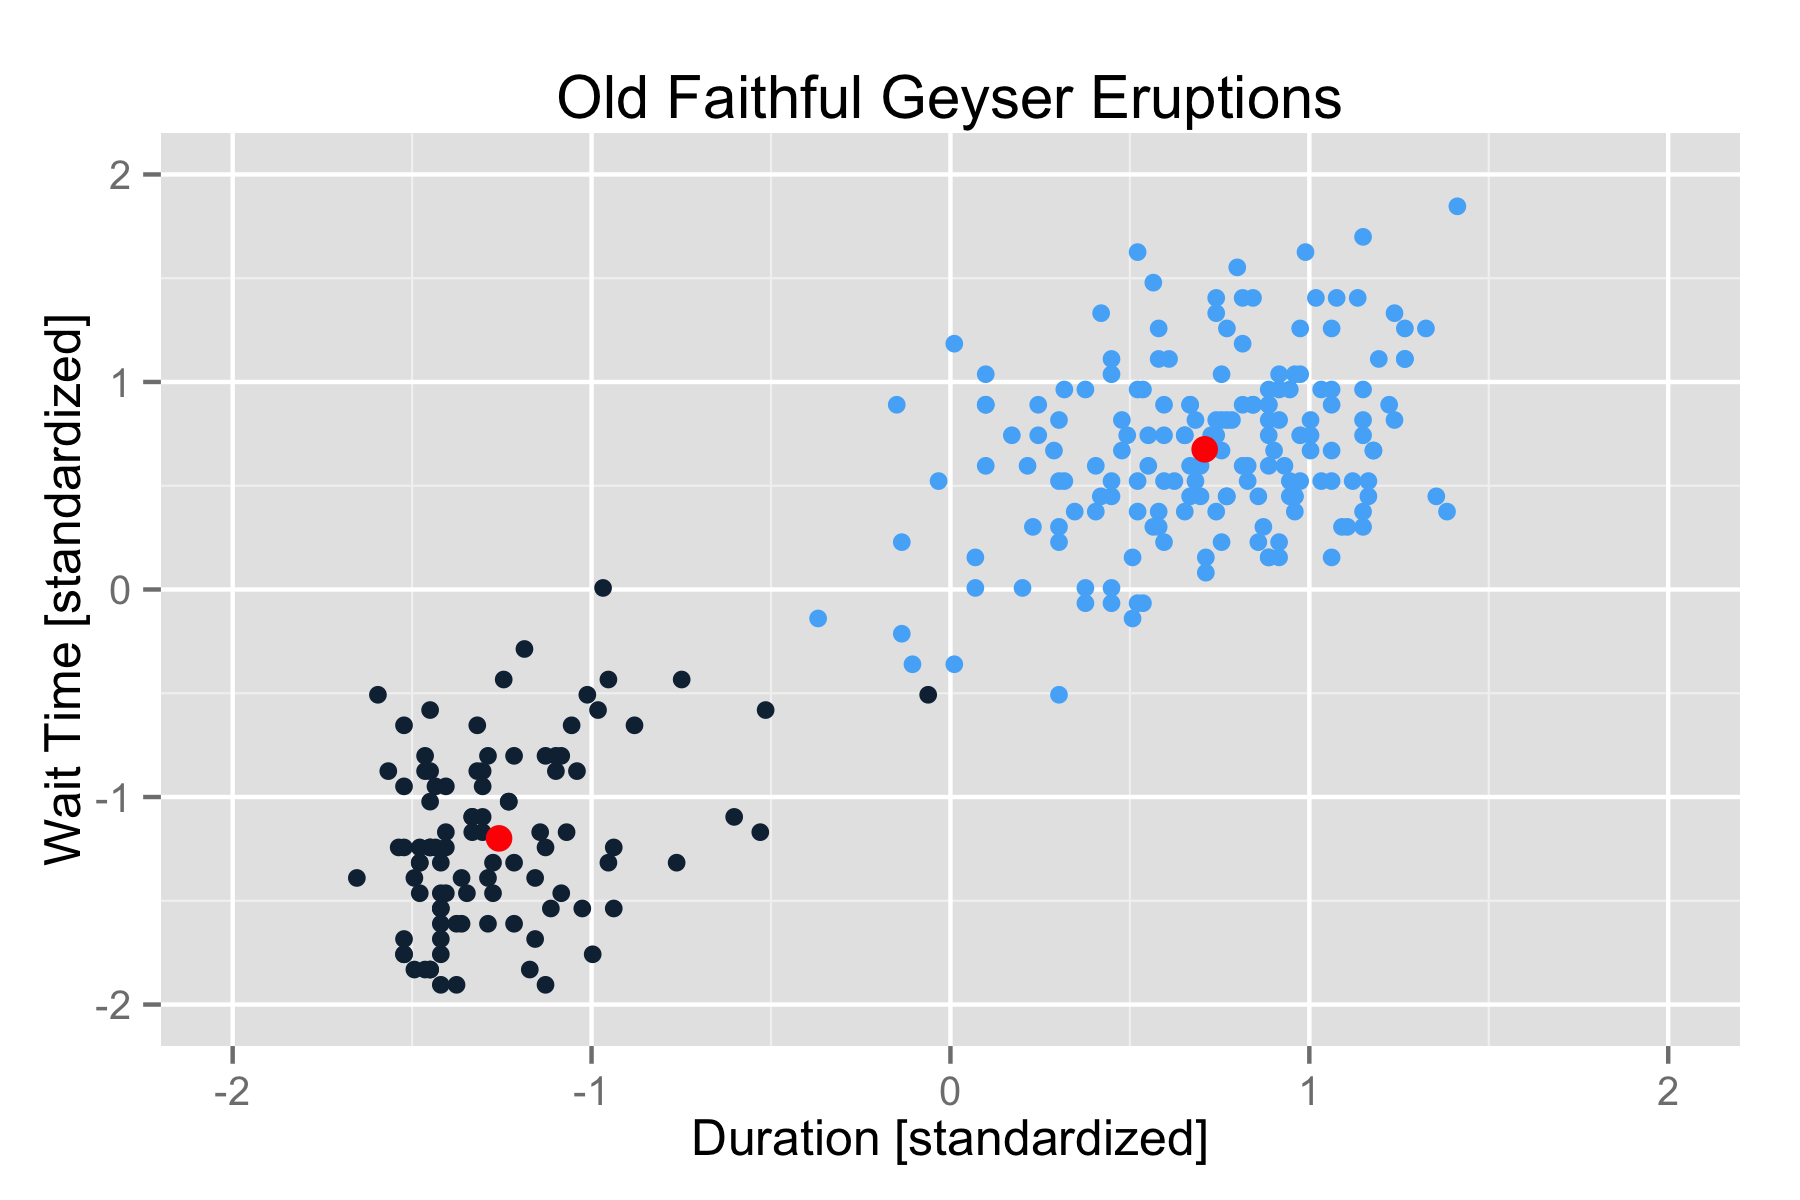
\includegraphics[width=0.65\textwidth]{../Figures/clustering/oldfaithful-clusterStandardize}
\par\end{center}
\begin{itemize}
\item Note several points have been reassigned from black to blue cluster.
\end{itemize}
\end{frame}

\begin{frame}{$k$-Means: Objective}
  \begin{itemize}
  \item Let $x_1,\ldots,x_n$ denote the data points and
    $\mu_1,\ldots,\mu_k$ the cluster points.
  \item Define the objective $\phi$ by
    $$\phi(x,\mu) = \sum_{i=1}^n \|x_i-\mu_{c(x_i)}\|_2^2,$$
    where $\mu_{c(x_i)}$ is the cluster point associated to~$x_i$.
  \item Then $\phi$ decreases at every round of $k$-means. Why?
    \pause
  \item Selecting mean of all associated data points improves objective.
  \item Selecting closest cluster point for each data points improves objective.
  \end{itemize}
\end{frame}

\section{$k$-Means: Failure Cases}
\begin{frame}{$k$-Means: Suboptimal Local Minimum}

\begin{itemize}
\item The clustering for $k=3$ below is a local minimum, but suboptimal:
\end{itemize}
\begin{center}
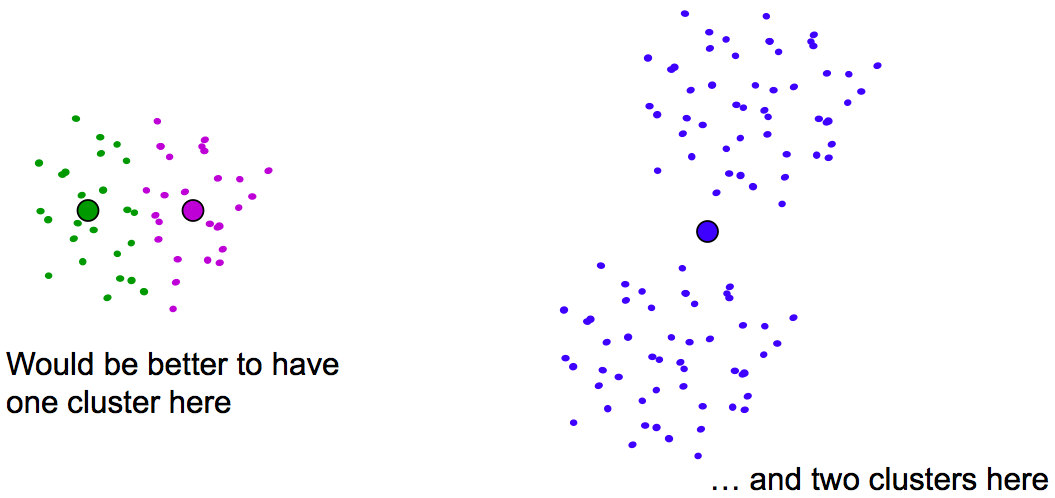
\includegraphics[width=0.8\textwidth]{../Figures/clustering/k-means-local-optimum}\let\thefootnote\relax\footnotetext{\tiny{From Sontag's DS-GA 1003, 2014, Lecture 8.}}
\par\end{center}

\end{frame}
\begin{frame}{$k$-Means$++$}

\begin{itemize}
\item Improvement on $k$-means by controlling the random
  initialization of the cluster centers.
\item Randomly choose first center amongst the data points.
\item For each of the remaining $k-1$ centers:
  \begin{itemize}
  \item Compute the distance from each data point to the closest
    already chosen center.
  \item Randomly choose a point as the new center with probability proportional
    to its computed distance squared.
  \end{itemize}
\item If we let $\phi$ denote the total sum of squares distances from
  each point to the closest cluster, then $k$-means$++$ has
  $$E[\phi]\leq 8(\log k+2)\phi_{\text{OPT}},$$
  where $\phi_{\text{OPT}}$ is from the optimal $k$-cluster assignment.
\end{itemize}
\end{frame}

\end{document}
